%% ========================================================================
%% chapter5.tex -- Chapter 5: Validation / Testing
%% Topic: Current-stage validation results for SAM-family polyp segmentation
%% Last updated: 2026-06-25
%% ========================================================================

\chapter{Validation and Results}
\label{chap:validation}

This chapter follows the ``Validation (or Testing)'' role in the BNBU partial-thesis template. Chapter~\ref{chap:solution} described how the benchmark was implemented; this chapter validates the current-stage benchmark by reporting quantitative trends, targeted metric evidence, and qualitative observations. The chapter does not select a single main model. Instead, it evaluates a current-stage benchmark and compares SAM-family adaptation strategies under the research questions defined in Chapter~\ref{chap:intro}.

\section{Validation Protocol and Interpretation Rules}
\label{sec:validation-protocol}

The primary validation protocol is the v3 protocol defined in Chapter~\ref{chap:outline}. V3-aligned baselines are evaluated on Kvasir-SEG \texttt{val.txt} with 120 held-out images and on the full CVC-ClinicDB set with 612 cross-domain images. The inference prompt is a fixed $\pm30$ pixel box derived from the ground-truth mask. Dice is used as the primary segmentation metric, but precision, recall, HD95, and FPS are used whenever the interpretation depends on over-segmentation, under-segmentation, boundary error, or efficiency.

The interpretation rules are equally important. ASPS is evaluated as a fully supervised external upper-bound reference on the PraNet held-out test set, so it is used for gap-to-reference analysis rather than direct v3 ranking. OP-SAM is reported as a one-shot, training-free, CPG-only exploratory pilot without the v3 ground-truth box prompt. Discarded exploratory models are not used as validation evidence in this partial thesis.

\section{RQ1: Foundation-Model Scaling}
\label{sec:rq1-results}

The first validation question asks whether larger foundation-model backbones improve zero-shot box-prompt polyp segmentation. The core comparison uses SAM v1 ViT-B/L/H and SAM2 Hiera-S/Base+/Large. The result is non-monotonic: SAM ViT-L is the strongest tested SAM v1 backbone, while SAM ViT-H does not further improve the result; SAM2 scaling follows a different pattern and does not provide a simple size-to-accuracy trend. This supports $H_1$: backbone scale must be validated per model family rather than assumed to improve segmentation automatically.

\begin{table}[H]
\centering
\caption{Core zero-shot backbone-scaling validation under the v3 protocol. Values are Dice scores.}
\label{tab:rq1-scaling-results}
\begin{tabular}{lccp{5.8cm}}
\toprule
\textbf{Family} & \textbf{Best Kvasir Dice} & \textbf{Best CVC Dice} & \textbf{Interpretation} \\
\midrule
SAM v1 & 0.8140 (ViT-L) & 0.6588 (ViT-L) & ViT-L is the strongest tested SAM v1 backbone; ViT-H does not improve further. \\
SAM2 & 0.7738 (Hiera-S) & 0.5754 (Hiera-L) & The scaling pattern differs across datasets and is not monotonic. \\
\bottomrule
\end{tabular}
\end{table}


\section{RQ2: Generic Medical Pre-Training Transfer}
\label{sec:rq2-results}

The second question asks whether generic medical pre-training improves zero-shot endoscopic polyp segmentation. The core comparison is SAM ViT-B versus MedSAM. MedSAM does not outperform vanilla SAM under the v3 protocol: its Kvasir Dice is lower, and its CVC Dice is essentially tied with SAM ViT-B. This supports $H_2$: medical pre-training alone does not guarantee transfer to colonoscopic polyps because the endoscopic domain differs from the mixed-modality data used to train generic medical SAM variants.

\begin{table}[H]
\centering
\caption{Medical-transfer validation under the v3 protocol.}
\label{tab:rq2-transfer-results}
\begin{tabular}{lccp{5.8cm}}
\toprule
\textbf{Method} & \textbf{Kvasir Dice} & \textbf{CVC Dice} & \textbf{Interpretation} \\
\midrule
SAM ViT-B & 0.7497 & 0.5182 & Generic zero-shot baseline. \\
MedSAM & 0.7034 & 0.5172 & Generic medical pre-training does not improve the v3 zero-shot result. \\
\bottomrule
\end{tabular}
\end{table}

\section{RQ3: K-Shot Adaptation Strategy}
\label{sec:rq3-results}

The third question compares full-encoder prompt-perturbation fine-tuning with rank-4 LoRA PEFT under the same K-shot support sizes. This is the central adaptation-strategy comparison of the current-stage benchmark, but it is not framed as a single main-method selection. The validation asks which adaptation strategy is more effective under a limited support budget and how the trend changes from in-domain to cross-domain evaluation.

\begin{table}[H]
\centering
\caption{K-shot adaptation trend under the v3 protocol. Values are Dice scores.}
\label{tab:rq3-kshot-results}
\begin{tabular}{lcccccc}
\toprule
\textbf{Method} & \textbf{Kvasir 1} & \textbf{Kvasir 5} & \textbf{Kvasir 10} & \textbf{CVC 1} & \textbf{CVC 5} & \textbf{CVC 10} \\
\midrule
PP-SAM & 0.7992 & 0.8512 & 0.8550 & 0.7516 & 0.8040 & 0.7709 \\
SAMed LoRA & 0.7456 & 0.7571 & 0.7230 & 0.5759 & 0.5747 & 0.5435 \\
\bottomrule
\end{tabular}
\end{table}

\begin{figure}[H]
\centering
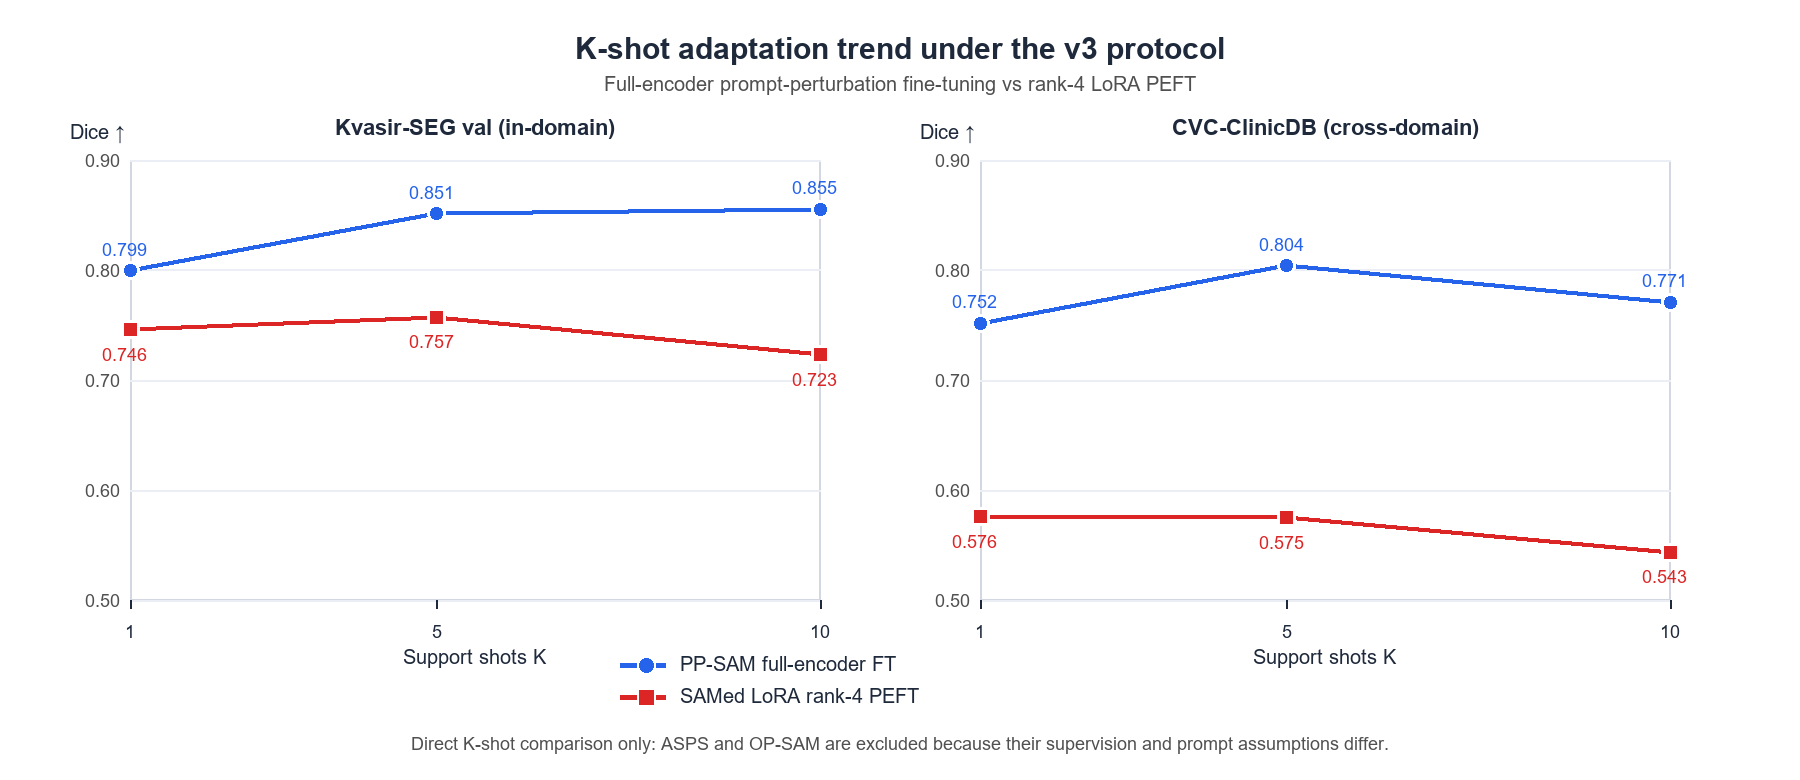
\includegraphics[width=0.95\textwidth]{figures/chapter5/fig_ch5_kshot_adaptation_trend.png}
\caption{K-shot adaptation trend for PP-SAM and SAMed LoRA. The comparison is restricted to v3-aligned K-shot adaptation methods with the same support sizes.}
\label{fig:ch5-kshot-trend}
\end{figure}

Figure~\ref{fig:ch5-kshot-trend} makes two trends visible. First, PP-SAM improves from 1-shot to 5-shot on both datasets, but 10-shot provides only a marginal Kvasir gain and reduces CVC Dice. This indicates that more support images do not automatically improve cross-domain generalisation. Second, SAMed LoRA remains weaker in the K-shot setting and does not show a stable gain as $K$ increases.

The secondary metrics explain part of this behaviour. SAMed LoRA K-shot runs maintain high recall but lower precision: for example, the 10-shot CVC run has recall 0.9892 but precision 0.3972. This indicates over-segmentation: the model often covers the polyp region but also includes too much background. Therefore, the K-shot LoRA weakness is not simply a failure to detect polyps; it is a mismatch between high recall and insufficient spatial precision.

\section{RQ4: Gap to Fully Supervised Upper-Bound Reference}
\label{sec:rq4-results}

The fourth question separates two dimensions that should not be conflated: data budget and parameter budget. PP-SAM 5-shot represents limited-data adaptation, SAMed LoRA full 880 represents full-data parameter-efficient adaptation, and ASPS represents an external fully supervised dense-reference model. The comparison is deliberately described as a gap-to-reference analysis. ASPS is not a directly ranked v3 baseline because the available checkpoint follows the PraNet supervised protocol, but it remains useful as an external upper-bound reference.

\begin{table}[H]
\centering
\caption{Gap to full supervision. ASPS is an external PraNet-held-out reference, not a v3-ranked baseline.}
\label{tab:rq4-upper-bound-results}
\begin{tabular}{lccp{5.6cm}}
\toprule
\textbf{Method} & \textbf{Kvasir Dice} & \textbf{CVC Dice} & \textbf{Role} \\
\midrule
PP-SAM 5-shot & 0.8512 & 0.8040 & Limited-data prompt-perturbation reference. \\
SAMed LoRA full 880 & 0.8955 & 0.8608 & Full-data PEFT bridge; full training data, lightweight parameter updates. \\
ASPS & 0.9093 & 0.9129 & External fully supervised upper-bound reference. \\
\bottomrule
\end{tabular}
\end{table}

\begin{figure}[H]
\centering
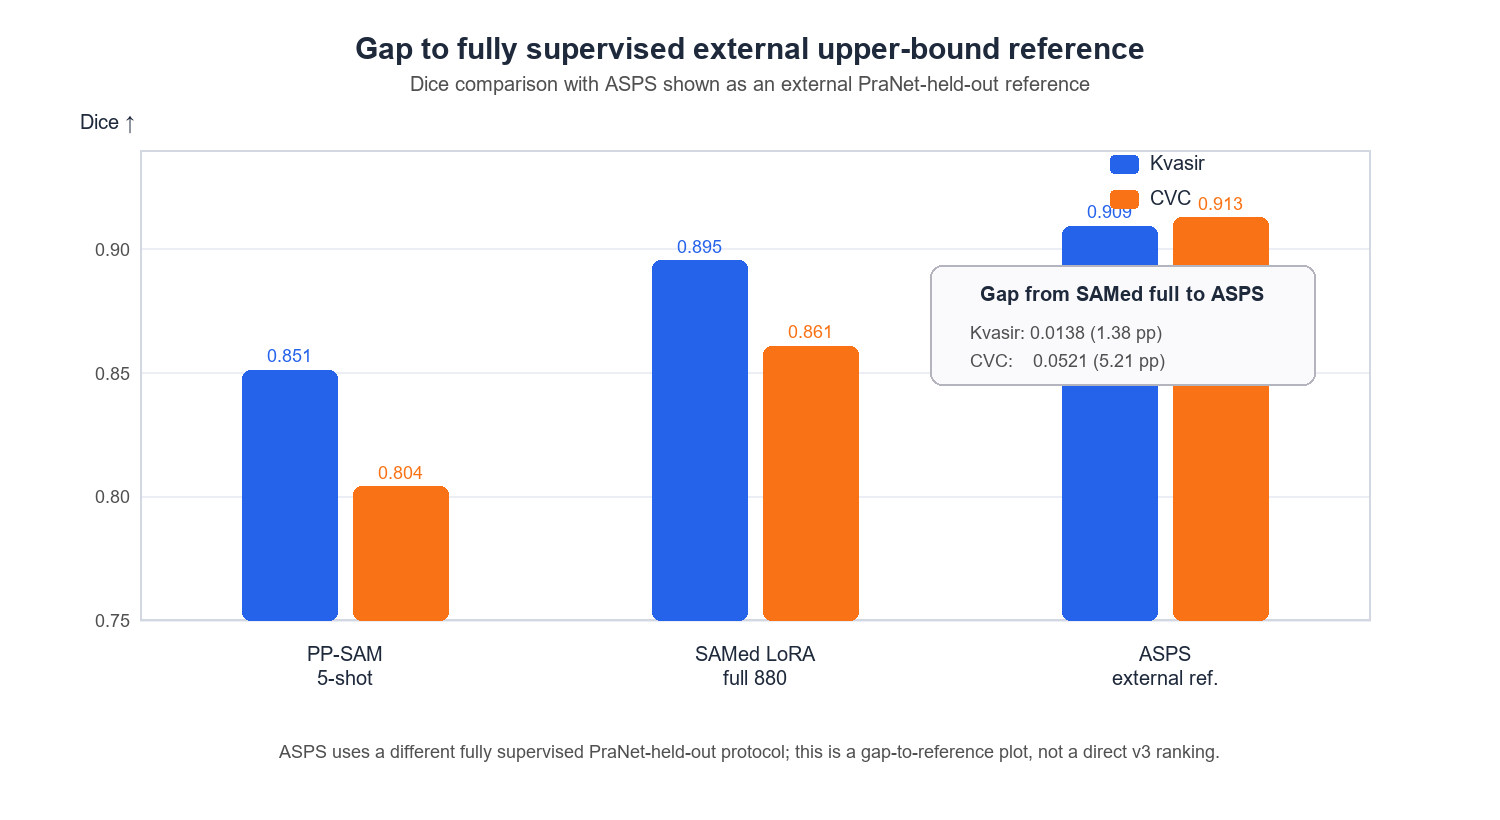
\includegraphics[width=0.82\textwidth]{figures/chapter5/fig_ch5_gap_to_upper_bound.png}
\caption{Gap from current-stage adaptation to the external fully supervised upper-bound reference. ASPS uses the PraNet held-out protocol and is therefore shown as a reference rather than a v3-ranked baseline.}
\label{fig:ch5-gap-upper-bound}
\end{figure}

SAMed LoRA full 880 narrows the gap to the external ASPS reference, but it should be read as full-data PEFT rather than as a few-shot result. The remaining Dice gap is 0.0138 on Kvasir and 0.0521 on CVC. This partially supports $H_4$: limited-data adaptation and full-data PEFT recover a substantial fraction of the external reference performance, but the cross-domain gap remains visible and cannot be treated as closed by the current-stage experiments.

\section{RQ5: Prompt-Free and Robustness Extensions}
\label{sec:rq5-results}

The fifth question records what remains unresolved beyond the current-stage benchmark. OP-SAM provides the current exploratory evidence for prompt-free, support-conditioned segmentation. Under the current CPG-only implementation, OP-SAM obtains 0.4373 Dice on Kvasir and 0.3719 Dice on CVC. These numbers are far below PP-SAM 1-shot, even though both settings consume one labelled support example. However, the assumptions differ: PP-SAM fine-tunes model parameters and consumes the v3 box prompt, while OP-SAM is training-free and generates its prompt from a support image.

The validation implication is therefore narrow and cautious. The current CPG-only OP-SAM pilot is not reliable enough to serve as a competitive prompt-free alternative in this benchmark. This does not prove that full OP-SAM fails, because the current implementation does not include SPF and EPE. Instead, it identifies full OP-SAM reproduction, prompt-quality ablation, object-scale stratification, and boundary-specific refinement as unresolved validation targets for the next phase.

\section{Qualitative Evidence and Failure-Mode Interpretation}
\label{sec:qualitative-failure-modes}

Qualitative evidence is useful when it explains what the metrics cannot show directly. In this thesis, qualitative examples should be read as representative outcomes under the benchmark rather than as evidence for selecting a final model. The existing PP-SAM qualitative stack illustrates the range from high-overlap cases to low-overlap cases, but it was generated from an earlier qualitative script. For that reason, it should be regenerated from the current v3 artifacts before being used as final evidence. The current validation therefore relies primarily on quantitative trends and targeted secondary metrics, while treating qualitative figures as supporting material.

\section{Validation Summary}
\label{sec:validation-summary}

The validation results support five current-stage conclusions. First, foundation-model scaling is family-specific and non-monotonic, so larger backbones do not automatically improve zero-shot polyp segmentation. Second, generic medical pre-training does not guarantee better transfer to endoscopic polyps under the current v3 validation protocol. Third, full-encoder prompt-perturbation fine-tuning is stronger than rank-4 LoRA in the K-shot setting, while LoRA becomes much more competitive with full 880-sample training. Fourth, current-stage adaptation approaches but does not close the gap to the external fully supervised ASPS reference. Fifth, prompt-free and robustness-oriented extensions remain open: CPG-only OP-SAM is exploratory, and systematic prompt-quality, object-scale, and boundary analyses are left for the next project phase.
